\NeedsTeXFormat{LaTeX2e}
\documentclass[a4paper,10pt,bibliography=totoc,oneside,openright,numbers=noenddot,headings=normal,DIV=9
%,draft
]{scrreprt}
\KOMAoptions{DIV=last}
\usepackage{scrhack}

\pagestyle{headings}
\usepackage[ngerman]{babel}
\usepackage[babel,german=quotes]{csquotes}
\usepackage[utf8]{inputenc}
\usepackage[T1]{fontenc}
\renewcommand{\sfdefault}{phv}
\renewcommand{\rmdefault}{phv}
\renewcommand{\ttdefault}{pcr}
\usepackage{graphicx}
\usepackage{verbatim}
\usepackage{tabularx}
\usepackage{subfigure}
\usepackage{url}
\usepackage{color}
\definecolor{LinkColor}{rgb}{0,0,0.2}
\usepackage{amssymb}
\usepackage{amsmath}
\usepackage{amsthm}
\usepackage{setspace}
\usepackage{fullpage} % or addmargin in cover
\usepackage{listings}
\lstset{language=Java,
  showstringspaces=false,
  frame=single,
  numbers=left,
  basicstyle=\ttfamily,
  numberstyle=\tiny}

% hier Namen etc. einsetzen
\newcommand{\fullname}{Tobias Dreher}
\newcommand{\email}{tobias.dreher@uni-ulm.de}
\newcommand{\titel}{Sprechererkennung}
\newcommand{\jahr}{2012}
\newcommand{\matnr}{123456}
\newcommand{\gutachterA}{Dr.\ Friedhelm Schwenker}
\newcommand{\betreuer}{Dipl.-Inf.\ Sascha Meudt}
\newcommand{\fakultaet}{Ingenieurwissenschaften\\und Informatik}
\newcommand{\institut}{Institut für Neuroinformatik}

%color in tables
\usepackage{colortbl}
\definecolor{Gray}{rgb}{0.80784, 0.86667, 0.90196} %dunkelblau
\definecolor{Lightgray}{rgb}{0.9176, 0.95, 0.95686} %hellblau
\definecolor{Akzent}{rgb}{0.6627, 0.63529, 0.55294} %akzentfarbe
\setlength{\arrayrulewidth}{0.1pt}

\clubpenalty10000
\widowpenalty10000

\setlength{\parindent}{0pt}
\setlength{\parskip}{1.4ex plus 0.35ex minus 0.3ex}

% Tiefe, bis zu der Überschriften in das Inhaltsverzeichnis kommen
\setcounter{tocdepth}{1}

\pdfinfo{
  /Author (\fullname)
  /Title (\titel)
  /Producer (PDFLaTeX)
  /Keywords ()
}

\usepackage{hyperref}
\hypersetup{
pdftitle=\titel,
pdfauthor=\fullname,
pdfsubject={Projekt},
pdfproducer={PDFLaTeX},
colorlinks=true,
	linkcolor=LinkColor,
	citecolor=LinkColor,
	filecolor=LinkColor,
	menucolor=LinkColor,
	urlcolor=LinkColor,
pdfborder=0 0 0	% keine Box um die Links!
}

%Trennungsregeln
\hyphenation{Sil-ben-trenn-ung}

\begin{document}
%\frontmatter

% Titelseite
\thispagestyle{empty}
%\begin{addmargin*}[-8mm]{8mm}
\vspace*{1.0em}


\includegraphics[height=1.8cm]{images/unilogo_bild}
\hfill

\includegraphics[height=1.8cm]{images/unilogo_wort}
\vspace*{2.1em}

{\footnotesize
{\bfseries Universität Ulm} \textbar ~89069 Ulm \textbar ~Germany
\hfill\parbox[t]{42mm}{\bfseries Fakultät für\\
\fakultaet\\
\mdseries \institut}
\vspace*{2cm}

\parbox{140mm}{\bfseries \huge \titel}

{\footnotesize Projekt an der Universität Ulm}
\vspace*{4em}

{\footnotesize
{\bfseries Vorgelegt von:}\\
\fullname\\\email\\[2em]
{\bfseries Gutachter:}\\
\gutachterA\\
[2em] %\gutachterB\\
{\bfseries Betreuer:}\\
\betreuer
\\[1.5em]
\jahr}
}
%\end{addmargin*}


% ab hier Zeilenabstand 1,4 fach 10pt/14pt
\setstretch{1.4}

\tableofcontents

%\mainmatter
\chapter{Einleitung}

\section{Motivation}

\section{Ziele}

\chapter{Theorie}
\label{cha:theorie}
Als Grundlage für die nachfolgenden Kapitel, wird in diesem Kapitel die Theorie hinter den verschiedenen Arbeitsschritten zur Sprechererkennung vorgestellt. Dies erfolgt in der Reihenfolge, wie die einzelnen Schritte verwendet werden. Die Reihenfolge geht aus dem Abschnitt \ref{sec:uebersicht} hervor.

\section{Übersicht}
\label{sec:uebersicht}
Die Sprechererkennung und auch Anwendungen wie Sprecherverfikation, Gesichtserkennung und Texterkennung, werden jeweils in vier Arbeitsschritte unterteilt. Diese sind \emph{Preprocessing}, \emph{Training} \emph{Prediction} und \emph{Analysis}. Diese werden wie in Abbildung \ref{fig:allgemeinerAblauf} dargestellt nacheinander ausgeführt. Beim Preprocessing (engl.: Vorverarbeitung) werden die Daten in das passende Format konvertiert, wichtige Informationen extrahiert und eventuell skaliert. Danach findet das Training durch einen Klassifikator oder ein künstliches neuronales Netz statt. Die Prediction (engl.: Vorhersage) ist die eigentliche Arbeitsphase der Erkennung. Anhand der trainierten Daten wird entschieden, welchem Sprecher die eingegeben Daten zugeordnet werden können. Der letzte Arbeitsschritt stellt die Analysis (engl. Analyse) dar. Hierdurch werden die Ergebnisse der Prediction verifiziert und evtl. auch visualisiert.

\begin{figure}[h]
  \centering
  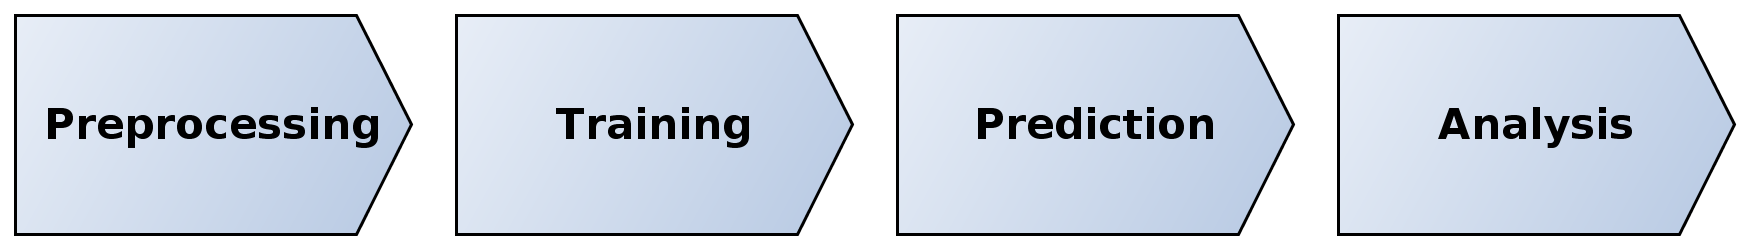
\includegraphics[width=0.85\textwidth]{images/allgemeinerAblauf}
  \caption{Einzelne Arbeitsschritte der Sprechererkennung}
  \label{fig:allgemeinerAblauf}
\end{figure}

\section{Preprocessing}
Der Schritt der Vorverarbeitung teilt sich in drei Teile auf: \emph{Konvertierung}, \emph{Feature Extraction} und \emph{Skalierung}. Diese drei Schritte werden in den folgenden Abschnitten genauer erläutert. Das Preprocessing ist von der Problemstellung abhängig. Bei der Sprechererkennung ist es die Verarbeitung von Audiostreams und die Abbildung auf die Stimm- und Hörorgane des Menschen.

\subsection{Konvertierung}
Mit der Konvertierung wird dafür gesorgt, dass die Daten im gleichen Format vorliegen. Für die Sprechererkennung reicht es, wenn die Audiodaten auf einen Kanal beschränkt werden (\emph{Mono}). Des Weiteren wird in dieser Projektarbeit eine Abtastrate von 16 kHz und einer Abtastgenauigkeit von 16 Bit verwendet.

\subsection{Feature Extraction}
Zur Extraktion von wichtigen Informationen werden zwei gängige Verfahren eingesetzt. Zum einen ist dies das Linear Predictive Coding (LPC). Beim LPC wird der Stimmtrakt des Menschen modellhaft nachgebildet. Dadurch wird die Datenbasis stark reduziert und werden nur die wichtigsten Informationen gespeichert.

Mel Frequency Cepstral Coefficients (MFCC)

\subsection{Skalierung}
Gelegentlich kann durch eine Skalierung der extrahierten Daten die Erkennung verbessert werden. Wahlweise kann zwischen $[0,1]$ oder $[-1,1]$ skaliert werden. Die Skalierung erfolgt linear nach der Formel \ref{equ:skalierung1} für $[0,1]$ und nach der Formel \ref{equ:skalierung2} für $[-1,1]$. $min$ stellt den kleinsten Wert der zu skalierenden Daten dar. $max$ den größten Wert. \cite{bib:svmfaq}
\begin{equation}
	\label{equ:skalierung1}
	x'=\frac{x-min}{max-min}
\end{equation}
\begin{equation}
	\label{equ:skalierung2}
	x'=2*\frac{x-min}{max-min}-1
\end{equation}

\section{Training}
Übersicht über Training, Weitere Möglichkeiten (K-Means, Kohonenkarten,...)
\subsection{Neural Gas}
Robustes Neuronales Netz
Nachbarschaftsreichweite
Update-Regel
\subsection{Support Vector Machine}
Support Vector Machine (SVM) ist ein (optimaler) Klassifikator
Eingesetzt wird Multi-Class SVM (One vs. One, One vs. Rest)

\section{Prediction}
Übersicht über Prediction, Erklärung Prediction = Arbeitsphase, erzeugt Ergebnis
\subsection{Nearest Neighbor}
Distanz zwischen Eingabevektor und Codebookvektoren
\subsection{Klassifikation}
Einordnung von Merkmalsvektoren

\section{Analysis}
Dient der Überprüfung des Ergebnisses der Prediciton-Phase evtl. mit Visualisierung\\
Möglichkeiten sind die absolute Erkennungsrate, Erkennungsrate auf mehrere Frames hintereinander, Verwechslungsmatrix

\chapter{Implementierung}
Das Ziel der Projektarbeit ist sowohl ein Offline- als auch ein Online-Modus zu implementieren und insbesondere mit dem Offline-Modus die eingesetzten Algorithmen zu vergleichen. Im diesem Kapitel werden die Kernmodule, die für beide Modi benötigt werden, sowie die einzelnen Modi beschrieben. Des Weiteren wird im letzten Abschnitt ein Evolutionärer Algortihmus zur Parameteroptimierung beschrieben.

\section{Kernmodule}
Der Kern sämtlicher Implementierungen stellen verschiedene Module dar, die für verschiedene Einsatzzwecke benutzt werden können. Bei jedem Modul handelt es sich um ein ausführbares Programm. In Abbildung \ref{fig:moduluebersicht} sind alle Kernmodule dargestellt. Gelb markiert sind die eigens für das Projekt in Java implementierten Module, blau markiert sind Module, die aus der \emph{libsvm} (Version 3.12) stammen. Die Kernmodule decken die in Kapitel \ref{cha:theorie} beschrieben vier Arbeitsschritte vollständig ab. 

\begin{description}
	\item[Preprocessing] Im Modul \emph{FeatureExtraction} werden die einkommenden Wav-Dateien (Mono, 16 kHz, 16 Bit) in Featurevektoren umgewandelt. Die Umwandlung erfolgt über LPC oder MFCC, wobei für MFCC die Bibliothek \emph{CoMIRVA} verwendet wird. \cite{bib:comirva} Für die Verwendung von SVM in Trainings- und Prediction-Phase ist eine Skalierung von Vorteil. Hierzu wird das Modul \emph{SvmScale} der \emph{libsvm} verwendet.
	\item[Training] Das Training kann auf zweierlei Arten durchgeführt werden. Zum einen wird durch das Modul \emph{SvmTrain} der \emph{libsvm} ein SVM-Klassifikator zur Verfügung gestellt. Zum anderen wird durch \emph{CreateCodebook} ein Codebuch auf Basis des Neural Gas Algorithmus erzeugt.
	\item[Prediction] Wurde beim Training SVM verwendet, wird in dieser Phase das Modul \emph{SvmPrediction} der \emph{libsvm} verwendet. Wurde dagegen ein Codebuch erstellt, wird die Methode des nächsten Nachbarn mit dem Modul \emph{NearestNeighbor} verwendet.
	\item[Analysis] Das Modul \emph{Analysis} wertet die Ergebnisse der Prediction-Phase aus und speichert sowohl die Erkennungsrate, als auch eine Verwechslungsmatrix in einer Ausgabedatei.
\end{description}

Zum Informationsaustausch zwischen den Modulen wird das bestehende Dateiformat der \emph{libsvm} benutzt. Dadurch ist die Interoperabilität mit der \emph{libsvm} gewährleistet, ohne dass ein Wrapper dafür benötigt wird.

\begin{figure}[h]
  \centering
  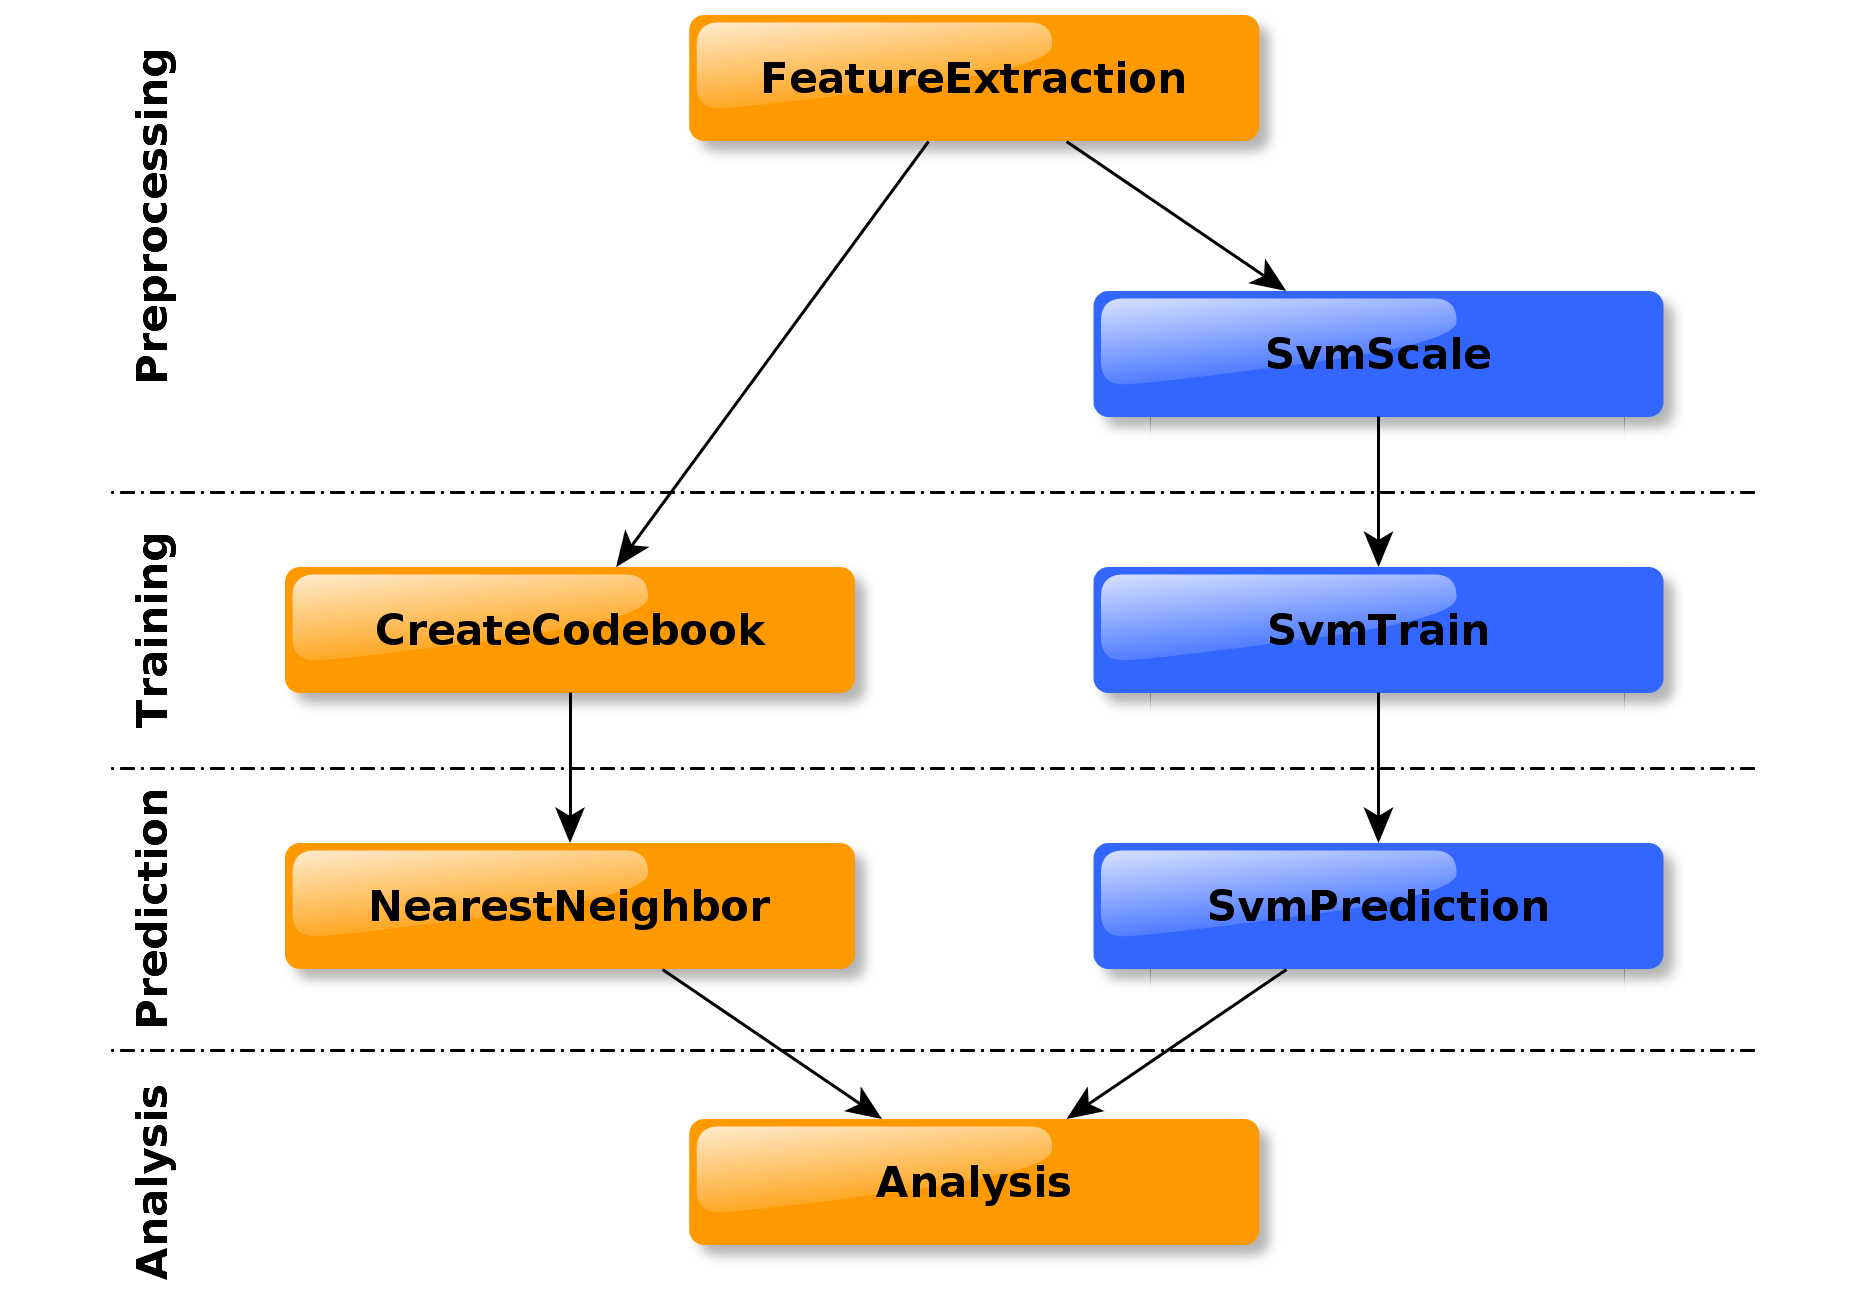
\includegraphics[width=1\textwidth]{images/moduluebersicht}
  \caption{Kernmodule in der Übersicht}
  \label{fig:moduluebersicht}
\end{figure}

Der Vorteil in der Modularisierung liegt in der flexiblen Anwendung. So kann beispielsweise unkompliziert getestet werden, ob die Skalierung auch beim Einsatz von \emph{Neural Gas} sinnvoll ist. Des Weiteren können die Module für weitere Einsatzzwecke genutzt werden. Um zum Beispiel eine Gesichts- oder Texterkennung zu implementieren müsste nur das \emph{FeatureExtraction}-Modul ausgetauscht werden. Der Nachteil einer solchen Modularisierung stellen die beschränkten Debuggingmöglichkeiten dar. Da es sich um für sich jeweils abgeschlossene Programme handelt, kann man nicht auf herkömmliche Weise im Programmcode debuggen.

\section{Offline-Test}
Ein Bash-Skript dient der Vergleichbarkeit der Ergebnisse. Dieses ermöglicht die Veränderung sämtlicher Einstellungen, wie die Fensterbreite der Featurevektoren oder der Trainingsmethode. Das Skript führt eine Kreuzvalidierung über drei Blöcke durch und speichert das Analyseergebnis in einer Datei.

\section{Online-Modus}
Ein Java-Programm stellt den Online-Modus der Sprechererkennung dar. Dieses verwendet MFCC in der Preprocessing-Phase und Neural Gas in der Trainingsphase. Diese Algorithmen werden verwendet, da sie zum Zeitpunkt der Implentation subjektiv am effizentisten arbeiteten. Das Programm ist so implementiert, dass es immer nach 320 ms ein Statusupdate auf der Konsole ausgibt. In diesem wird der Sprecher über die letzten 1,6 Sekunden ermittelt, wobei neuere Werte stärker gewichtet werden. Die einzelnen Gewinner der neuesten Feature-Vektoren werden 5-fach so stark gewichtet, wie die der ältesten Feature-Vektoren. Die Gewichtung nimmt linear mit dem Alter der Feature-Vektoren ab.

\section{Evolutionärer Algorithmus zur Parameteroptimierung}
Betrachtet man die einstellbaren Parameter für MFCC und Neural, ergibt dies einen 7-dimensionalen Vektorraum in dem das Optimum der Parameter gefunden werden soll. Die einzelnen Parameter sind:
\begin{itemize}
	\item Fensterbreite
	\item Überlappung der Fenster
	\item Merkmale pro Fenster
	\item Minmale Energielevel
	\item Fensterfunktion (Hamming oder Hann)
	\item Größe des Codebuchs
	\item Iterationen des Neural Gas Algorithmus
\end{itemize}
Sollte die Fensterbreite veränderbar sein, lassen sich die Ergebnisse nur noch schwer vergleichen, da mit der Fensterbreite auch die Information pro Fenster steigt. Somit wurde diese Einstellung auf 32 ms Fensterbreite fixiert.

Um das Optimum in dem noch verbleibenden 6-dimensionalen Vektorraum zu finden, dient ein Evolutionärer Algorithmus. Dabei wird eine variable Mutationsrate eingesetzt, da diese lokale Optimas besser vermeidet, als eine statitische Mutationsrate. Die Fitnessfunktion stellt die Funktion \ref{equ:fitness} dar. Als Eingabeparameter dienen der Funktion die für den Durchlauf mit den aktuellen Parametern benötigte Zeit in Sekunden $t$, sowie die Erkennungsrate auf Einzelfenster in Prozent $acc$. Zur Selektion dient eine Tournament-Selektion, bei de je vier Individuen gegen einander antreten, wobei nur der beste in die nächste Population gelangt. Eine Population besteht aus 12 Individuen. 

\begin{equation}
	\label{equ:fitness}
	\begin{aligned}[t]f(t,acc) = \frac{acc}{1 - e^{\left(\frac{-t}{1000}\right)}}\end{aligned}
\end{equation}

\chapter{Ergebnisse}
Übersicht über Ergebnisse

\section{Offline-Modus}
Übersicht über Offline-Modus

\subsection{Standardwerte}
10 Sprecher\\
Eingesetzte Standardwerte sind: (Tabelle?)\\
Feature Extraction
\begin{itemize}
	\item 32 ms Fenster
	\item Halber Vorschub
	\item 90 \% Energielevel
	\item 12 Merkmale (LPC) bzw. 20 Merkmale (MFCC)
\end{itemize}
Neural Gas
\begin{itemize}
	\item 100 Prototypen
	\item 15 Iterationen
\end{itemize}
SVM
\begin{itemize}
	\item RBF oder linearer Kernel
	\item $\gamma$ = 1
	\item c = 1
\end{itemize}

\subsection{Vergleich der Algorithmen}
\begin{tabular}{l|c|c}			
	& LPC & MFCC \\
	\hline
	Neural Gas & 40 \% & 71 \% \\
	SVM (linear) & 46 \% & 72 \% \\
	SVM (RBF) & 54 \% & 80 \% \\
\end{tabular}
Verwechslungsmatrixen
		
\subsection{Optimierung durch Evolutionären Algorithmus}
Bilder der Optimierung\\
Pareto Front (Bild)\\
Ergebnisse:
\begin{itemize}
	\item MFCC
	\begin{itemize}
		\item 32 ms Fenster (fix)
		\item 100 \% -> 20 \% Vorschub
		\item 96 \% -> 85 \% Energielevel
		\item 25 - 33 Merkmale
	\end{itemize}
	\item Neural Gas
	\begin{itemize}
		\item 53 -> 176 Prototypen
		\item 5 -> 9 Iterationen
	\end{itemize}
\end{itemize}

\section{Online-Modus}
Nicht in Zahlen zu fassen, da kein Test vorhanden ist. Allerdings werden nur mittelmäßige Erkennungsraten erreicht, die von den Sprechern und den Mikrophonen abhängig zu sein scheinen.

\chapter{Diskussion}

\section{Offline-Modus}

\section{Online-Modus}


\appendix
% hier Anhänge einbinden
%\input{chapters/sources}

%\backmatter

%\bibliographystyle{plaindin} % Nummern und alphabetisch sortiert
%\bibliographystyle{alphadin} % Buchstaben und sortiert
%\bibliographystyle{abbrvdin} % Nummern und abgekürzte Namen
\bibliographystyle{unsrtdin} % Nummern und unsortiert
\bibliography{bibliography}


%\clearpage
%\thispagestyle{empty}

%Name: \fullname \hfill Matrikelnummer: \matnr \vspace{2cm}

%\minisec{Erklärung}

%Ich erkläre, dass ich die Arbeit selbständig verfasst und keine anderen als die angegebenen Quellen und Hilfsmittel verwendet habe.\vspace{2cm}

%Ulm, den \dotfill

%\hspace{10cm} {\footnotesize \fullname}
\end{document}
